\documentclass[tikz]{standalone}
\usepackage{cancel}
\usepackage{fontspec}
\setmonofont[Scale=MatchLowercase]{DejaVu Sans Mono}
\usetikzlibrary{arrows.meta}

\begin{document}
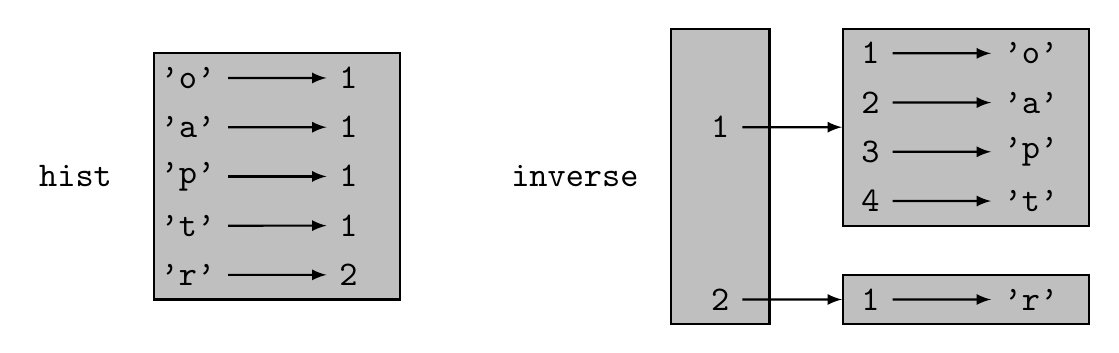
\begin{tikzpicture}[thick, scale=1.25, transform shape]
$\node[anchor=east](h) at(-1.55, 0) {\tt hist};
\node[draw, fill=lightgray, minimum width=2.5cm, minimum height=2.5cm](hv) at(0,0){};
\node[anchor=east](o) at (-0.5, 1) {\tt 'o'};
\node[anchor=west](ov) at (0.5, 1) {\tt 1};
\draw[-latex] (o)--(ov);
\node[anchor=east](a) at (-0.5, 0.5) {\tt 'a'};
\node[anchor=west](av) at (0.5, 0.5) {\tt 1};
\draw[-latex] (a)--(av);
\node[anchor=east](p) at (-0.5, 0) {\tt 'p'};
\node[anchor=west](pv) at (0.5, 0) {\tt 1};
\draw[-latex] (p)--(pv);
\node[anchor=east](t) at (-0.5, -0.5) {\tt 't'};
\node[anchor=west](tv) at (0.5, -0.5) {\tt 1};
\draw[-latex] (t)--(tv);
\node[anchor=east](r) at (-0.5, -1) {\tt 'r'};
\node[anchor=west](rv) at (0.5, -1) {\tt 2};
\draw[-latex] (r)--(rv);
\node[anchor=east](i) at(3.8, 0) {\tt inverse};
\node[draw, fill=lightgray, minimum width=1cm, minimum height=3cm](iv) at(4.5,0){};
\node(n1) at(4.5,0.5){\tt 1};
\node(n2) at(4.5,-1.25){\tt 2};
\node(a1) [draw, fill=lightgray, minimum width=2.5cm, minimum height=2cm] at(7,0.5){};
\node(a2) [draw, fill=lightgray, minimum width=2.5cm, minimum height=0.5cm] at(7,-1.25){};
\draw[-latex](n1)--(a1);
\draw[-latex](n2)--(a2);
\node[anchor=east](t1) at(6.25, 1.25){\tt 1};
\node[anchor=east](t2) at(6.25, 0.75){\tt 2};
\node[anchor=east](t3) at(6.25, 0.25){\tt 3};
\node[anchor=east](t4) at(6.25, -0.25){\tt 4};
\node[anchor=east](tt1) at(6.25, -1.25){\tt 1};
\node[anchor=west](v1) at(7.25, 1.25){\tt 'o'};
\node[anchor=west](v2) at(7.25, 0.75){\tt 'a'};
\node[anchor=west](v3) at(7.25, 0.25){\tt 'p'};
\node[anchor=west](v4) at(7.25, -0.25){\tt 't'};
\node[anchor=west](vv1) at(7.25, -1.25){\tt 'r'};
\draw[-latex](t1)--(v1);
\draw[-latex](t2)--(v2);
\draw[-latex](t3)--(v3);
\draw[-latex](t4)--(v4);
\draw[-latex](tt1)--(vv1);
$
\end{tikzpicture}
\end{document}
